\documentclass[journal,12pt,twocolumn]{IEEEtran}

\usepackage{setspace}
\usepackage{gensymb}
\singlespacing
\usepackage[cmex10]{amsmath}

\usepackage{amsthm}

\usepackage{mathrsfs}
\usepackage{txfonts}
\usepackage{stfloats}
\usepackage{bm}
\usepackage{cite}
\usepackage{cases}
\usepackage{subfig}
\usepackage{tasks}

\usepackage{longtable}
\usepackage{multirow}

\usepackage{amsthm}

\usepackage{enumitem}
\usepackage{mathtools}
\usepackage{steinmetz}
\usepackage{tikz}
\usepackage{circuitikz}
\usepackage{verbatim}
\usepackage{tfrupee}
\usepackage[breaklinks=true]{hyperref}
\usepackage{graphicx}
\usepackage{tkz-euclide}

\usetikzlibrary{calc,math}
\usepackage{listings}
    \usepackage{color}                                            %%
    \usepackage{array}                                            %%
    \usepackage{longtable}                                        %%
    \usepackage{calc}                                             %%
    \usepackage{multirow}                                         %%
    \usepackage{hhline}                                           %%
    \usepackage{ifthen}                                           %%
    \usepackage{lscape}     
\usepackage{multicol}
\usepackage{chngcntr}

\DeclareMathOperator*{\Res}{Res}

\renewcommand\thesection{\arabic{section}}
\renewcommand\thesubsection{\thesection.\arabic{subsection}}
\renewcommand\thesubsubsection{\thesubsection.\arabic{subsubsection}}

\renewcommand\thesectiondis{\arabic{section}}
\renewcommand\thesubsectiondis{\thesectiondis.\arabic{subsection}}
\renewcommand\thesubsubsectiondis{\thesubsectiondis.\arabic{sub subsection}}


\hyphenation{optical networks semiconduc-tor}
\def\inputGnumericTable{}                                 %%

\lstset{
%language=C,
frame=single, 
breaklines=true,
columns=fullflexible
}
\date{March 2021}

\begin{document}

\newcommand{\BEQA}{\begin{eqnarray}}
\newcommand{\EEQA}{\end{eqnarray}}
\newcommand{\define}{\stackrel{\triangle}{=}}
\bibliographystyle{IEEEtran}
\raggedbottom
\setlength{\parindent}{0pt}
\providecommand{\mbf}{\mathbf}
\providecommand{\pr}[1]{\ensuremath{\Pr\left(#1\right)}}
\providecommand{\qfunc}[1]{\ensuremath{Q\left(#1\right)}}
\providecommand{\fn}[1]{\ensuremath{f\left(#1\right)}}
\providecommand{\e}[1]{\ensuremath{E\left(#1\right)}}
\providecommand{\sbrak}[1]{\ensuremath{{}\left[#1\right]}}
\providecommand{\lsbrak}[1]{\ensuremath{{}\left[#1\right.}}
\providecommand{\rsbrak}[1]{\ensuremath{{}\left.#1\right]}}
\providecommand{\brak}[1]{\ensuremath{\left(#1\right)}}
\providecommand{\lbrak}[1]{\ensuremath{\left(#1\right.}}
\providecommand{\rbrak}[1]{\ensuremath{\left.#1\right)}}
\providecommand{\cbrak}[1]{\ensuremath{\left\{#1\right\}}}
\providecommand{\lcbrak}[1]{\ensuremath{\left\{#1\right.}}
\providecommand{\rcbrak}[1]{\ensuremath{\left.#1\right\}}}
\theoremstyle{remark}
\newtheorem{rem}{Remark}
\newcommand{\sgn}{\mathop{\mathrm{sgn}}}
\providecommand{\abs}[1]{\vert#1\vert}
\providecommand{\res}[1]{\Res\displaylimits_{#1}} 
\providecommand{\norm}[1]{\lVert#1\rVert}
%\providecommand{\norm}[1]{\lVert#1\rVert}
\providecommand{\mtx}[1]{\mathbf{#1}}
\providecommand{\mean}[1]{E[ #1 ]}
\providecommand{\fourier}{\overset{\mathcal{F}}{ \rightleftharpoons}}
%\providecommand{\hilbert}{\overset{\mathcal{H}}{ \rightleftharpoons}}
\providecommand{\system}{\overset{\mathcal{H}}{ \longleftrightarrow}}
	%\newcommand{\solution}[2]{\textbf{Solution:}{#1}}
\newcommand{\solution}{\noindent \textbf{Solution: }}
\newcommand{\cosec}{\,\text{cosec}\,}
\providecommand{\dec}[2]{\ensuremath{\overset{#1}{\underset{#2}{\gtrless}}}}
\newcommand{\myvec}[1]{\ensuremath{\begin{pmatrix}#1\end{pmatrix}}}
\newcommand{\mydet}[1]{\ensuremath{\begin{vmatrix}#1\end{vmatrix}}}
\numberwithin{equation}{subsection}
\makeatletter
\vspace{3cm}
\title{Assignment 4}
\author{Suraj - CS20BTECH11050}
\maketitle
\newpage
\bigskip
\renewcommand{\thetable}{\theenumi}
\newcommand{\dsum}{\displaystyle\sum}
\newcommand{\comb}[2]{{}^{#1}\mathrm{C}_{#2}}
\newcommand{\R}{\mathbb{R}}
\newcommand{\C}{\mathbb{C}}
\newtheorem{theorem}{Theorem}[section]
\newtheorem{lemma}[theorem]{Lemma}
\newtheorem{definition}{Definition}
Download all python codes from 
\begin{lstlisting}
https://github.com/Suraj11050/Assignments-AI1103/tree/main/Assignment%204/Python%20codes
\end{lstlisting}
%https://www.overleaf.com/project/604c4c718ee4e22400cf9d22
Download Latex-tikz codes from 
%
\begin{lstlisting}
https://github.com/Suraj11050/Assignments-AI1103/blob/main/Assignment%204/Assignment%204.tex
\end{lstlisting}
\section{GATE 2021 (ST), Q.17 (STATISTICS SECTION)} 
If the marginal probability density function of the $k^{th}$ order statistic of a 
random sample of size 8 from a uniform distribution on $[0,2]$ is
\[
  f(x) =
  \begin{cases}
   \dfrac{7}{32}\,x^{6}\,\brak{2-x},  & 0<x<2, \\ 
      \hspace{1cm}   0,               & \text{otherwise,} 
  \end{cases}
\]
then $k$ equals \underline{\hspace{3cm}}
\bigskip
\section{SOLUTION}
Let $X\in[0,2]$ be a random variable of uniform order statistic distribution of sample size 8 then
\begin{align}
 \int_{0}^{2} \pr{x}\,dx &= 1 \\
 \pr{x}                  &= \dfrac{1}{2}\;\brak{\because \text{Uniform order}}
\end{align}
The PDF for X is 
\begin{align}
\fn{x} = 
 \begin{cases}
  \dfrac{1}{2},      &0<x<2, \\ 
     0, &\text{otherwise,}
 \end{cases} \label{d}
\end{align}
 The CDF for X is 
 
 \begin{align}
 F(x) = 
 \begin{cases}
  \dfrac{x}{2},      &0<x<2, \\ 
     0, &\text{otherwise,}
 \end{cases} \label{e}
 \end{align}
 
\newpage

\begin{definition}
$k^{th}$ order statistic : If the sample is arranged in an ascending order, the $k^{th}$ order statistic is the $k^{th}$ element from the left.$\;X_{(k)}$ is called $k^{th}$ vector of order statistic  
For a sample $\{X_1, X_2, \cdots X_n\}$ of size n:
\begin{align}
\nonumber  X_{(1)} &= \min{\{X_1, X_2, \cdots X_n\}}\\
\nonumber  X_{(n)} &= \max{\{X_1, X_2, \cdots X_n\}} \\
\nonumber  X_{(1)} &\leq X_{(2)}\leq \cdots\leq X_{(k)}\leq \cdots \leq X_{(n)} 
\end{align}
\end{definition}

\bigskip

Let $X_{(k)}$ be vector of order statistic of $(X_1,X_2\cdots,X_n)$ 
 \begin{lemma}
 Marginal probability density (PDF) for a $k_{th}$ order statistic of a random sample of size n given CDF$=F(x)$ and
 PDF$=\fn{x}$ is given by 
 \begin{align}
\nonumber f_{(k,n)}(x) = n\,\comb{n-1}{k-1}\,\brak{1-F(x)}^{n-k}F(x)^{k-1} f(x)
 \end{align}                                                \label{1}
 \end{lemma}
 
\begin{proof}
 The CDF of the $k^{th}$ order statistic from a sample of size n is:
\begin{align}
\nonumber F_{(k,n)}(x) &= \pr{X_{(k)}\leq x} \\
                       &= \dsum_{j=k}^{n}\,\comb{n}{j}\,\brak{1-F(x)}^{n-j} F(x)^{j}
\end{align}
 
Deriving PDF of $k^{th}$ order statistic from a sample of size n:
 
 \begin{align}
\nonumber \dfrac{d}{dx} F_{(k,n)}(x) &= \dfrac{d}{dx}\brak{\dsum_{j=k}^{n}\,\comb{n}{j}\,\brak{1-F(x)}^{n-j} F(x)^{j}} 
 \end{align}
\begin{multline}
\nonumber f_{(k,n)}(x) = \dsum_{j=k}^{n}\,\comb{n}{j}\,\brak{j}\brak{1-F(x)}^{n-j}F(x)^{j-1}\,f(x)  \\
                -\dsum_{j=k}^{n}\,\comb{n}{j}\,\brak{n-j}\brak{1-F(x)}^{n-j-1}F(x)^{j}\,f(x) 
\end{multline}
\begin{align}
S_1  &= \dsum_{j=k}^{n} \dfrac{n!}{(n-j)!\,(j-1)!}\brak{1-F(x)}^{n-j}F(x)^{j-1} f(x) \\
S_2  &= \dsum_{j=k}^{n}\,\dfrac{n!}{(n-j-1)!\,j!}\brak{1-F(x)}^{n-j-1}F(x)^{j}\,f(x) \label{a}
\end{align}
let $i = j+1$ change the limits for the summation in equation \eqref{a}
\begin{align}
\nonumber S_2  &= \dsum_{i=k+1}^{n}\,\dfrac{n!}{(n-i)!\,(i-1)!}\brak{1-F(x)}^{n-i}F(x)^{i-1}\,f(x)  
\end{align}
\begin{multline}
S_1 - S_2  =  \\
           \dfrac{n!}{(n-k)!\,(k-1)!}\brak{1-F(x)}^{n-k}F(x)^{k-1} f(x) 
\end{multline}

\begin{align}
f_{(k,n)}(x) &= n\,\comb{n-1}{k-1}\,\brak{1-F(x)}^{n-k}F(x)^{k-1} f(x) \label{b}
\end{align}
\end{proof}

Using Lemma \eqref{1} given $n=8$ substituting n, equation \eqref{d} and equation \eqref{e}  in above equation \eqref{b} we get:

\begin{align}
\nonumber f_{(k,n)}(x) &= 8\,\comb{7}{k-1}\,\brak{1-\dfrac{x}{2}}^{8-k}\brak{\dfrac{x}{2}}^{k-1} \dfrac{1}{2} \\
f_{(k,n)}(x) &= \dfrac{1}{32}\,\comb{7}{k-1}\,\brak{2-x}^{8-k}\,x^{k-1} \label{c} 
\end{align}
Comparing the marginal probability density function obtained in equation \eqref{c} with the equation given in question
\begin{align}
\nonumber \dfrac{1}{32}\,\comb{7}{k-1}\,\brak{2-x}^{8-k}\,x^{k-1} &= \dfrac{7}{32}\,\brak{2-x}\,x^6 \\
\therefore k &= 7 
\end{align}
Hence the marginal probability density in the given problem is $7^{th}$ order uniform statistic and \textbf{the value of k is 7}
\newpage
\begin{figure}[htp]
    \centering
    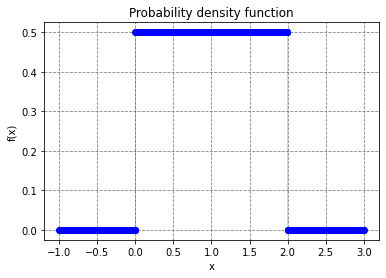
\includegraphics[width = \columnwidth]{PDF.png}
    \label{fig:PDF  of X}
\end{figure}
\begin{figure}[htp]
    \centering
    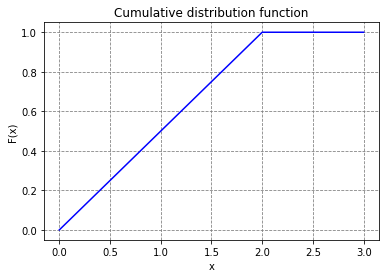
\includegraphics[width = \columnwidth]{CDF.png}
    \label{fig:CDF of X}
\end{figure}
\end{document}
